\documentclass[english,version-2020-11]{uzl-thesis}


\UzLThesisSetup{
  Masterarbeit,
  Logo-Dateiname        = {uzl-thesis-logo-itcs.pdf},
  Verfasst              = {am}{Institut für Theoretische Informatik},
  Titel auf Deutsch     = {Über elementare Eigenschaften einer mehrdimensionalen Verallgemeinerung des euklidischen Algorithmus},
  Titel auf Englisch    = {On Elementary Properties of a Multi-Dimensional Generalization of the Euclidean Algorithm},
  Autor                 = {Daniel Knaack},
  Betreuerin            = {Prof. Dr. Kim-Manuel Klein},
  Studiengang           = {Informatik},
  Datum                 = {18. Juni 2024},
  Abstract              = {TODO},
  Zusammenfassung       = {TODO},
  Numerische Bibliographie,
}

\UzLStyle{alegrya modern design}

\begin{document}

\chapter{Introduction}

\chapter{Preliminaries}

\section{Generalized Euclidean Algorithm}

\begin{Pseudocode}
while $x$ is not integral do
  solve $Bx = c$
  find $x_l$ which is not integral
  swap $B_l$ and $c$
  ...
end
\end{Pseudocode}

\chapter{Bounds}

\section{What Makes a Bad Solution?}

In one dimension, a solution is bad when the value $x_1$ is close to $1$.
However, in the next iteration $x_1$ would be close to $0$ and therefore
would lead to a greater decrease in the determinant.
An initial guess would be that the solution lies exactly between $0$ and $1$ at $1/2$.
However, this solution is also good as after just one step we have achieved integrality.

The solution is to choose a value $x_1$ such that its value in the first
iteration is the same as its value in the second iteration.
This means we are trying to solve the following equation:
\[
  x_1 = 1/x_1 - 1.
\]
This gives us the polynomial $x^2 + x - 1$ where the root is the inverse of the
golden ratio.

% TODO: Explore other strategies. Can we generalize this to every possible strategy?
In just two dimensions, we already have an additional degree of freedom.
Since the solution $x$ consists of two values, we can choose which index we pivot with.
We will choose the value with the smallest fractional value as this decreases
the determinant the fastest.
We assume w.l.o.g. that our values are sorted in increasing order.
This means we pivot with $x_1$ first.

% TODO: What about just choosing the golden ratio for every x_i?
% TODO: Are odd dimensions easier since the decrease is not worse? We could
% choose two values to be the same, since the ratio for odd dimensions is
% smaller than the previous dimension
Just like in one dimension we want to choose $x_1$ carefully such that the
determinant decreases the same amount in every iteration.
A simple solution would be to fill both values with the golden ratio.
In this case, it does not matter which index we choose as each one decreases
the determinant the same amount.
However, in two dimensions we can make this decrease slightly worse
by choosing different values for $x_1$ and $x_2$ such that we swap the pivot
in each iteration.

Assuming the value for $x_1$ is already chosen where would $x_2$ be placed?
Ideally, it would be close to the right side of $x_1$, because then the new
value $-x_2 / x_1$ would be close to $-1$ and the fractional value would be
close to $1$.
Since the decrease must stay the same in each iteration, this gives us the
following two equations:
\begin{align*}
  x_1 = 2 - x_2 / x_1 \\
  x_2 = 1 / x_1 - 1,\\
\end{align*}
which leads to the following polynomial:
\begin{align*}
  x_1^3 - 2x_1^2 - x_1 + 1 = 0
\end{align*}

Let $\phi_2$ be the root of this polynomial.
If we choose $x_1 = \phi_2$ and $x_2 = 2\phi_2 - \phi_2^2$,
then the values in the second iteration are
\[\begin{aligned}
  x_1' & = 1 / x_1 - 1   &  & = 1 / \phi_2 - 1                    &  & = 2\phi_2 + \phi_2^2 &  & = x_2, \\
  x_2' & = 2 - x_2 / x_1 &  & = 2 - (2\phi_2 + \phi_2^2) / \phi_2 &  & = \phi_2             &  & = x_1
\end{aligned}\]

We can extend this to $d$ dimensions using the following equations:
\begin{align*}
  x_1 = 2 - x_2 / x_1 \\
  x_2 = 2 - x_3 / x_1 \\
  x_3 = 2 - x_4 / x_1 \\
  \vdots \\
  x_{d-1} = 2 - x_d / x_1 \\
  x_d = 1 / x_d - 1 \\
\end{align*}

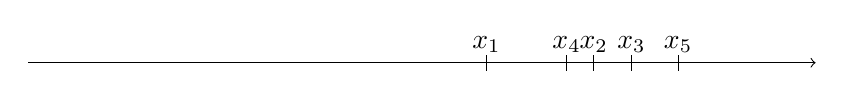
\begin{tikzpicture}[scale=10]
  \draw (0.5820216424559055, -0.01) -- node[above] {$x_1$} (0.5820216424559055, 0.01);
  \draw (0.7181491667223714, -0.01) -- node[above] {$x_2$} (0.7181491667223714, 0.01);
  \draw (0.7661126076135922, -0.01) -- node[above] {$x_3$} (0.7661126076135922, 0.01);
  \draw (0.6837042616132034, -0.01) -- node[above] {$x_4$} (0.6837042616132034, 0.01);
  \draw (0.8252940926247403, -0.01) -- node[above] {$x_5$} (0.8252940926247403, 0.01);
  \draw[->] (0, 0) -- (1, 0);
\end{tikzpicture}

\section{Fibonacci Numbers}

\begin{itemize}
  \item Fibonacci numbers are just linear recurrences with constant coefficients $c_0 = 1, c_1 = 1$.
  \item Linear recurrence with coefficients $c_0, c_1, \dots, c_d$: $a_{n+d+1} = \sum_{i=0}^d c_i a_{n+i}$.
  \item The characteristic polynomial of the Fibonacci sequence is the polynomial of the golden ratio.
  \item For even dimensions: $c_0 = -1, c_1 = 1, c_2 = 2, c_3 = -2, \dots, c_{2d-1} = -2, c_{2d} = 2$.
  \item For odd dimensions:  $c_0 = 1, c_1 = -1, c_2 = -2, c_3 = 2, \dots, c_{2d} = -2, c_{2d+1} = 2$.
  \item The ratio $\phi_d$ for the characteristic polynomials approaches $1/\sqrt{3}$ as $d \to \infty$.
  \item Folding an A4 paper?
\end{itemize}

\chapter{$d$-bonacci Number}

\section{Multi-Dimensional Golden Ratio}

\begin{definition}[$d$-dimensional Golden Ratio]
  The $d$-dimensional golden ratio is the only positive real root $\phi_d$ of the polynomial:
  \[
    x^{d+1} + x^d + \dots + x^2 + x = 1.
  \]
\end{definition}

All sums of the form $\sum_{k=1}^i \phi_d^k$ with $i \le d$ must be strictly less than one.

Dividing by $x$ on each side gives us the following equation:
\[
  x^d + x^{d-1} + \dots + x + 1 = 1/x.
\]

% TODO: Explain why we can subtract one from each.
We choose $x_i = \sum_{k = 1}^i \phi_d^k$.
The values are ordered such that $x_1$ is the smallest value.
Therefore we begin pivoting with $x_1$.
After the update, the new value for $x_1$ is
\[
  x_1' = 1/\phi_d - 1 = \phi_d^d + \phi_d^{d-1} + \dots + \phi_d = x_d.
\]
The other values of the new solution are
\[
  x_i' = x_i / x_1 - 1 = \sum_{k = 1}^i \phi_d^k / \phi_d - 1 = \sum_{k=1}^{i-1} \phi_d^k.
\]
Hence, we rotate the values forwards, so that $x_i' = x_{i-1}$ and $x_1' = x_d$.
In the next iteration we would choose $x_2$ as our pivot since it is the smallest value.

\section{Higher-Order Fibonacci Numbers}

\begin{definition}
  The \emph{$d$-bonacci numbers} are defined as follows:
  \begin{enumerate}
    \item $F_d(0) = F_d(1) = \dots = F_d(d) = 0$.
    \item $F_d(n) = \sum_{i = 1}^{d+1} F_d(n - i)$ for $n > d$.
  \end{enumerate}
\end{definition}

Using the $d$-bonacci numbers, we can approximate the golden ratio $\phi_d$
by computing the ratio between consecutive terms $F_d(n - 1) / F_d(n)$.
Furthermore, we can approximate powers of the golden ratio by increasing the distance between the terms.
For example, we can approximate $\phi_d^2$ by the term $F_d(n - 2) / F_d(n)$.

In order to prove that the ratios approximate $\phi_d$,
we first prove the convergence criteria for this sequence, i.e.
the sequence is bounded and is monotonically increasing.

\begin{lemma}
  The ratio $F_d(n - i) / F_d(n)$ is bounded between $0$ and $1$.
\end{lemma}

\begin{proof}

\end{proof}

\begin{lemma}
  The ratios are monotonically increasing with increasing $n$.
\end{lemma}

\begin{proof}

\end{proof}

\begin{theorem}
  $\lim_{n \to \infty} F_d(n - k) / F_d(n) = \phi_d^i$ for $i \ge 1$.
\end{theorem}

\begin{proof}
  We begin with $k = 1$.
  By the previous lemmas, we can assume that the ratio approaches some limit $L$:
  \begin{align*}
    \lim_{n \to \infty} \frac{F_d(n - 1)}{F_d(n)} = L.
  \end{align*}
  From the definition of the $d$-bonacci numbers, we can rewrite $F_d(n - 1)$ as follows:
  \begin{align*}
    F_d(n) & = F_d(n - 1) + \dots + F_d(n - d - 1) \\
    \Leftrightarrow F_d(n - 1) & = F_d(n) - F_d(n - 2) - \dots - F_d(n - d - 1)
  \end{align*}
  This gives us the following equation for the limit $L$:
  \begin{align*}
    L = \lim_{n \to \infty} \frac{F_d(n - 1)}{F_d(n)}
      = \lim_{n \to \infty} 1 - \frac{\sum_{i=2}^{d+1} F_d(n - i)}{F_d(n)}
      = 1 - \sum_{i=2}^{d+1} \lim_{n \to \infty} \frac{F_d(n - i)}{F_d(n)}
  \end{align*}
  Each term in the sum can be rewritten as the ratio of two consecutive $d$-bonacci numbers:
  \begin{align}
    \label{eq:power}
    \lim_{n\to\infty} \frac{F_d(n - i)}{F_d(n)} = \lim_{n\to\infty}\frac{F_d(n - i)}{F_d(n - i + 1)} \cdot \ldots \cdot \frac{F_d(n - 1)}{F_d(n)} = L^i.
  \end{align}
  Therefore, as $n$ approaches infinity each term in the sum approaches a power of $L$:
  \begin{align*}
    L = \lim_{n \to \infty} \frac{F_d(n - 1)}{F_d(n)}
      = 1 - \sum_{i=2}^{d+1} \lim_{n \to \infty} \frac{F_d(n - i)}{F_d(n)}
      = 1 - L^2 - L^3 - \dots - L^{d+1}
  \end{align*}
  Per definition, the solution to this equation is exactly $\phi_d$.
  The limit for $k > 1$ follows directly from Equation~\ref{eq:power}.
\end{proof}

Using this theorem, we can swap out the power-sum of $\phi_d$ in the solution
vector from the previous section with sums of consecutive $d$-bonacci terms.
We set $x_i = \sum_{k=1}^i (-1)^k F_d(n - k) / F_d(n)$ and pivot with $x_1$.
The new value for $x_1$ is
\[
  x_1'
  = \{1/x_1\}
  = \frac{F_d(n)}{F_d(n - 1)} - 1
  = \sum_{k=1}^{d+1} (-1)^{k + 1} \frac{F_d(n - k)}{F_d(n - 1)} - 1
  = \sum_{k=1}^d (-1)^k \frac{F_d(n - 1 - k)}{F_d(n - 1)}
\]
and the new values for $x_i$ are
\[
  x_i'
  = -x_i / x_1
  = -\sum_{k=1}^i (-1)^k \frac{F_d(n - i)}{F_d(n)} \frac{F_d(n)}{F_d(n - 1)}
  = \sum_{k=1}^{i-1} (-1)^k \frac{F_d(n - 1 - i)}{F_d(n - 1)}.
\]

% TODO: How would we choose the matrix? Can

\chapter{Bounds (old)}

\begin{itemize}
  \item We choose the smallest index in each iteration since this gives us the
    largest change in the determinant.
\end{itemize}

Assumption:
\[
  x_1 = \frac{x_2}{x_1} - 1 = \dots = \frac{x_{d}}{x_{d-1}} - 1 = \frac{1}{x_d} - 1,
\]
which leads to the following polynomials:
\begin{align}
  \label{eq:solution}
  x_d^{d+1} + x_d - 1 = 0 \quad \text{ and } \quad x_i = x_d^{d - i + 1}.
\end{align}

In one dimension, the root of the polynomial $\phi_1$ is the \emph{inverse of the golden ratio}.
In two dimension, the root of the polynomial $\phi_2$ is the \emph{inverse of the supergolden ratio}.
Hence, we have to substitute $x$ with the inverse of $y$ to get the actual golden ratio:

\begin{align*}
  (1/y)^{d+1} + 1/y - 1       & = 0 \quad \text{(Expand second term with $y^d$)} \\
  1/y^{d+1} + y^d/y^{d+1} - 1 & = 0 \quad \text{(Multiply with $y^d$)}           \\
  1 + y^d - y^{d+1}           & = 0 \quad \text{(Multiply with $-1$)}            \\
  y^{d+1} - y^d - 1           & = 0                                              \\
\end{align*}

Let $\phi_d$ be the root of this polynomial.
For $d = 1$, the root $\phi_1$ is the \emph{golden ratio}.
For $d = 2$, the root $\phi_2$ is the \emph{supergolden ratio}.

The golden ratio can be approximated using the Fibonacci sequence,
the super golden ratio can be approximated using Narayana's cow sequence:

\begin{align*}
  F(0) = F(1) = 1,        & \quad F(n) = F(n - 1) + F(n - 2), n \ge 2 \\
  N(0) = N(1) = N(2) = 1, & \quad N(n) = N(n - 1) + N(n - 3), n \ge 3
\end{align*}

From the Narayana sequence, we can naturally generalize the sequence to higher dimensions:

\[
  F_d(0) = 0, F_d(1) = \dots = F_d(d) = 1, \quad F_k(n) = F_d(n - 1) + F_d(n - d - 1).
\]

\begin{table}[t]
  \caption{The first 18 Fibonacci numbers of orders one to five.}
  \begin{tabular}{c|cccccccccccccccccccc}
    $n$     & 0 & 1 & 2 & 3 & 4 & 5 & 6 & 7  & 8  & 9  & 10 & 11 & 12  & 13  & 14  & 15  & 16  & 17   \\ %& 18   & 19   \\
    \hline
    $d = 1$ & 0 & 1 & 1 & 2 & 3 & 5 & 8 & 13 & 21 & 34 & 55 & 89 & 144 & 233 & 377 & 610 & 987 & 1597 \\ %& 2584 & 4181 \\
    $d = 2$ & 0 & 1 & 1 & 1 & 2 & 3 & 4 & 6  & 9  & 13 & 19 & 28 & 41  & 60  & 88  & 129 & 189 & 277  \\ %& 406  & 595  \\
    $d = 3$ & 0 & 1 & 1 & 1 & 1 & 2 & 3 & 4  & 5  & 7  & 10 & 14 & 19  & 26  & 36  & 50  & 69  & 95   \\ %& 131  & 181  \\
    $d = 4$ & 0 & 1 & 1 & 1 & 1 & 1 & 2 & 3  & 4  & 5  & 6  & 8  & 11  & 15  & 20  & 26  & 34  & 45   \\ %& 60   & 80   \\
    $d = 5$ & 0 & 1 & 1 & 1 & 1 & 1 & 1 & 2  & 3  & 4  & 5  & 6  & 7   & 9   & 12  & 16  & 21  & 27   \\ %& 34   & 43   \\
  \end{tabular}
\end{table}

Any two consecutive terms can be used to approximate the corresponding ratio, i.e. $\lim_{n \to \infty} F_d(n) / F_d(n + 1) = \phi_d$.

Going back to the Euclidean algorithm,
an example matrix which leads to the solution given by Equation~\ref{eq:solution} is:
\begin{align*}
  \left(\begin{array}{ccccc|c}
    a^d    & 0       & \cdots & 0      & 0      & b^d     \\
    0      & a^{d-1} & \cdots & 0      & 0      & b^{d-1} \\
    \vdots & \vdots  & \ddots & \vdots & \vdots & \vdots  \\
    0      & 0       & \cdots & a^2    & 0      & b^2     \\
    0      & 0       & \cdots & 0      & a      & b       \\
  \end{array}\right),
\end{align*}
where $a = F_d(n)$ and $b = F_d(n + 1)$.

\begin{definition}
  The $d$-th golden ratio $\phi^{(d)}$ is the real positive root of $x^{d+1} - x^d - 1$.
\end{definition}

\begin{definition}
  The $d$-Fibonacci numbers are defined as follows:
  \begin{itemize}
    \item $F^{(d)}_0 = F^{(d)}_1 = \dots = F^{(d)}_{d-1} = 1$,
    \item $F^{(d)}_{n} = F^{(d)}_{n-1} + F^{(d)}_{n-d-1}$ for $n \ge d$.
  \end{itemize}
\end{definition}

\begin{lemma}
  The sequence $R^{(d)}_{n+d}$ can be reformulated as follows:
  \begin{align*}
    R^{(d)}_{n+d}
    & = 1 + \frac{1}{R^{(d)}_{n+d-1} R^{(d)}_{n+d-2} \dots R^{(d)}_n}
  \end{align*}
\end{lemma}

\begin{proof}
  \begin{align*}
    R^{(d)}_{n+d}
    & = \frac{F^{(d)}_{n+d+1}}{F^{(d)}_{n+d}}
    = \frac{F^{(d)}_{n+d} + F^{(d)}_{n}}{F^{(d)}_{n+d}}
    = 1 + \frac{F^{(d)}_{n}}{F^{(d)}_{n+d}} \\
    & = 1 + \frac{F^{(d)}_{n}}{R^{(d)}_{n+d-1} F^{(d)}_{n+d-1}}
    = 1 + \frac{F^{(d)}_{n}}{R^{(d)}_{n+d-1} R^{(d)}_{n+d-2} F^{(d)}_{n+d-2}} \\
    & \mathrel{\vdots} \\
    & = 1 + \frac{F^{(d)}_{n}}{R^{(d)}_{n+d-1} R^{(d)}_{n+d-2} \dots R^{(d)}_n F^{(d)}_n} \\
    & = 1 + \frac{1}{R^{(d)}_{n+d-1} R^{(d)}_{n+d-2} \dots R^{(d)}_n}
    \qedhere
  \end{align*}
\end{proof}

\begin{lemma}
  The sequence $R^{(d)}_n = F^{(d)}_{n+1} / F^{(d)}_{n}$ is bounded between $1$ and $2$.
\end{lemma}

\begin{proof}
  For all $n < d - 1$ this is obviously the case.
  Per induction, assume that $R^{(d)}_n, R^{(d)}_{n+1}, \dots, R^{(d)}_{n+d-1}$ are bounded.
  From the previous lemma, we know
  \begin{align*}
    R^{(d)}_{n+d}
    & = 1 + \frac{1}{R^{(d)}_{n+d-1} R^{(d)}_{n+d-2} \dots R^{(d)}_n}
  \end{align*}
  By the induction hypothesis, each ratio is bounded between $1$ and $2$.
  Therefore, $R^{(d)}_{n+d}$ is equally bounded between $1$ and $2$.
\end{proof}

\begin{lemma}
  The sequence $R^{(d)}_n$ is monotonically increasing.
\end{lemma}

\begin{proof}

\end{proof}

\begin{theorem}
  The sequence $R^{(d)}_n$ converges to $\phi^{(d)}$.
\end{theorem}

\begin{proof}
  From the previous two lemmas, we know that the sequence converges.
  Therefore, there exists some $L$ such that
  \[
    \lim_{n \to \infty} R^{(d)}_n = \lim_{n \to \infty} 1 + \frac{1}{R^{(d)}_{n-1} R^{(d)}_{n-2} \dots R^{(d)}_{n-d}} = L.
  \]
  As $n$ approaches infinity, all ratios approach some limit $L$.
  Hence, $L = 1 + 1/L^d$ or equivalently $L^{d+1} - L^d - 1 = 0$,
  which fits the definition of the golden ratio $\phi^{(d)}$.
\end{proof}

\chapter{Implementation}

\section{Using an Out-of-the-Box Solver}

\begin{itemize}
  \item Algorithm technically only requires one fractional bit to determine how to round.
  \item Problem: Solving a system of linear equations requires exact fractional solutions.
    Using floating-point numbers leads to inaccurate results.
  \item Could be solved by using an iterative method? However, does a method
    exist, which is accurate up to one fractional bit?
\end{itemize}

\section{Custom Implementation}

\begin{itemize}
  \item Uses custom \texttt{ratio} datatype which implements rational numbers.
  \item Linear system solver implemented using Gaussian elimination and pivoting.
  \item Only the basic algorithm is implemented, so far.
\end{itemize}

\begin{bibtex-entries}
\end{bibtex-entries}

\end{document}
